\subsection{Square-line picking}
\label{sec:square_line}

Here we consider choosing lines from a unit square, where the
end-points are chosen IID uniformly from the square. Generalization to
larger squares can be done by scaling (see Section~\ref{sec:scaling}),
or by using the rectangle-line pick1ing solution (see
Section~\ref{sec:rectangle_line}).

Figure~\ref{fig:square_eg} shows an example, and
Figures~\ref{fig:square_pdf} and show \ref{fig:square_cdf} the PDF and
CDF, respectively. 

\begin{figure}[tbp]
  \begin{center}
    \subfloat[\label{fig:square_eg}Square example.]
       {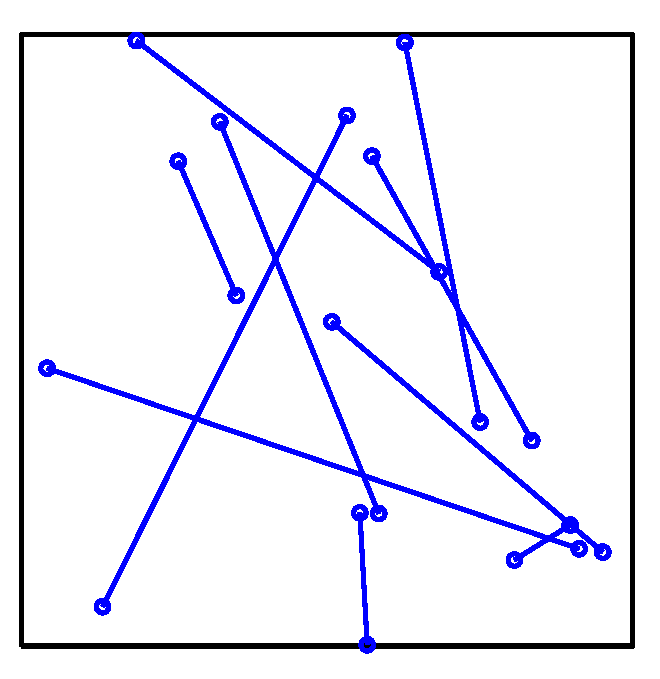
\includegraphics[width=0.18\columnwidth]{../Matlab/Plots/LinePicking_eg_square.eps}} 
    \hspace{3mm}
    \subfloat[\label{fig:square_pdf}PDF.]
       {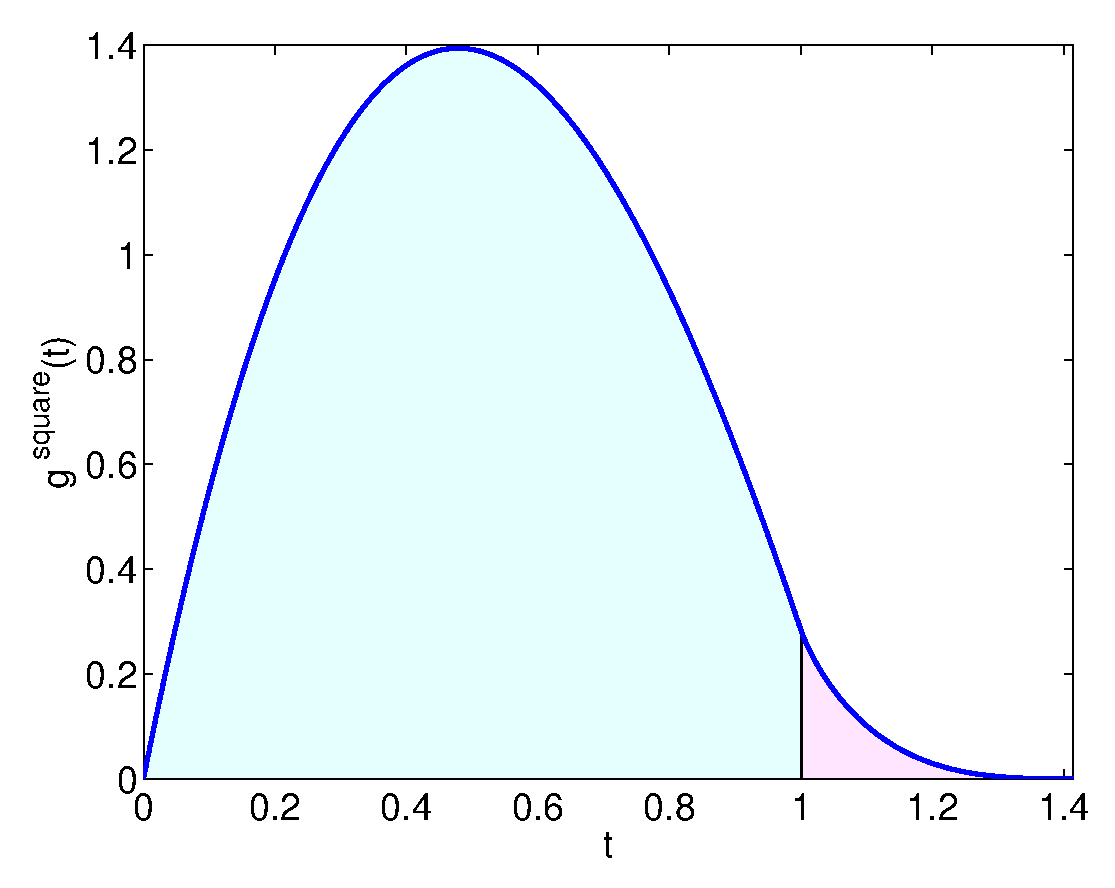
\includegraphics[width=0.4\columnwidth]{../Matlab/Plots/LinePicking_plot_square_pdf.eps}}
    \subfloat[\label{fig:square_cdf}CDF.]
       {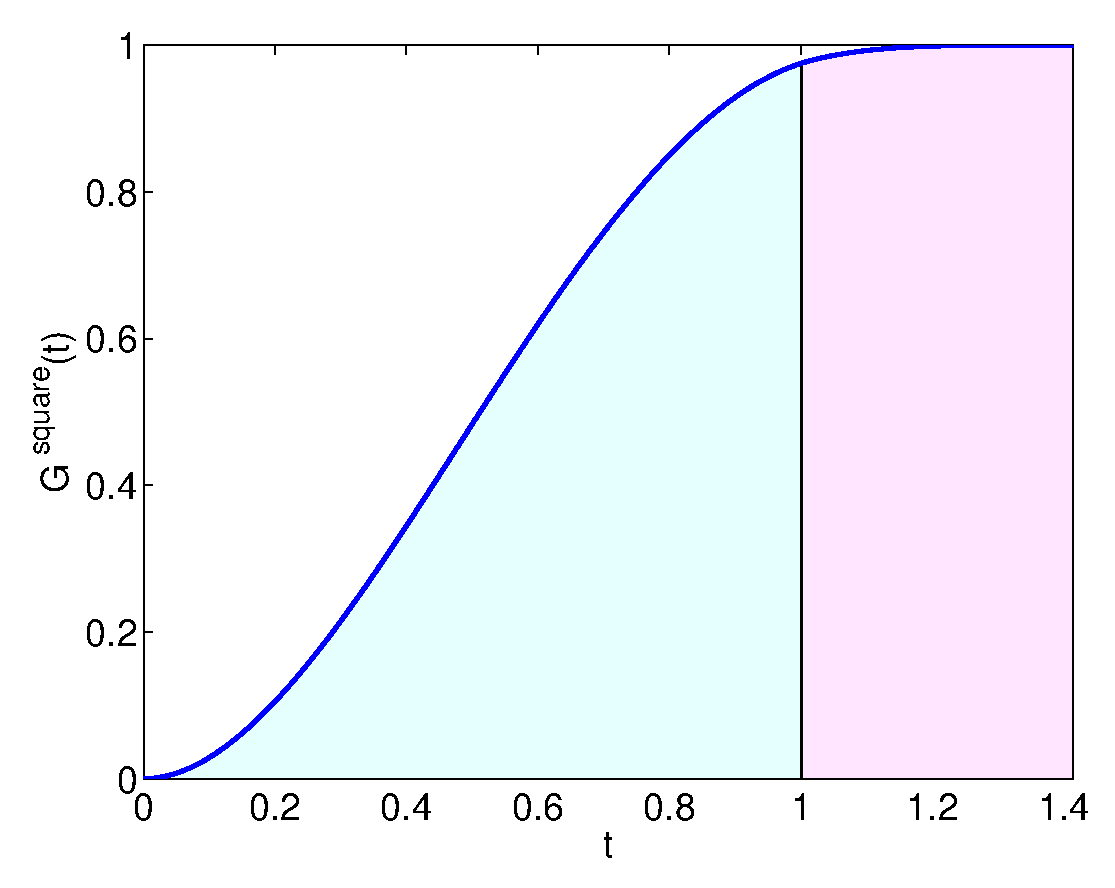
\includegraphics[width=0.4\columnwidth]{../Matlab/Plots/LinePicking_plot_square_cdf.eps}}
    \caption{The square-line picking problem.}
  \end{center} 
\vspace{-4mm}
\end{figure}

\subsubsection{PDF}

The PDF for the square is given in
\cite{philip:_probab_distr_distan_between_two,weisstein:_squar_line_picking},
but which is also a special case of the PDF for the rectangle
\eqref{eqn:rectangle} with $a=b$.
\begin{equation}
  \label{eq:square_line}
  g^{\rm square}(t) = \left\{ \begin{array}{ll}
      2t (t^2-4t+\pi), & \mbox{ for } 0 \leq t \leq 1, \\
      2t \left[4 \sqrt{t^2-1} - (t^2+2-\pi) - 4 \tan^{-1} \left(\sqrt{t^2-1} \right)\right], 
               & \mbox{ for } 1 \leq t \leq \sqrt{2} . \\ 
    \end{array} \right.
\end{equation}
% http://mathworld.wolfram.com/SquareLinePicking.html

\subsubsection{CDF}


\subsubsection{Moments}


